\documentclass[sigconf,natbib=false]{acmart}

\usepackage{tikz}
\usetikzlibrary{arrows.meta,positioning,shapes.geometric,fit,backgrounds}
\usepackage{pgfplots}
\pgfplotsset{compat=1.17}
\usepackage{algorithm}
\usepackage{algpseudocode}
\usepackage{booktabs}
\usepackage{listings}
\usepackage{xcolor}
\usepackage{amsmath,amssymb}
\usepackage{url}
\usepackage{xurl}
\sloppy

\lstdefinestyle{prompt}{
  basicstyle=\ttfamily\scriptsize,
  breaklines=true,
  frame=single,
  columns=fullflexible,
  backgroundcolor=\color{gray!8}
}

% ACM boilerplate switched off / replaced by EDBT macros
\settopmatter{printacmref=false}
\renewcommand\footnotetextcopyrightpermission[1]{}
\input{edbt-macros}
\microtypesetup{expansion=false,protrusion=true}

\begin{document}

\title{Cost-Bounded Cascaded Query Execution over Structured and Unstructured Movie Data}
\subtitle{Reconciling Predicate Pushdown and Batched Semantic Joins with Calibrated Two-Stage Cascades}

\author{Anna}
\affiliation{%
  \institution{Universit\'e Grenoble Alpes}
  \city{Grenoble}
  \country{France}
}
\email{anna@example.edu}

\begin{abstract}
Answering natural-language questions that mix structured predicates (e.g.\ release year, film duration, genre) with unstructured predicates over free text (e.g.\ ``the reviews are strongly negative'') requires a query engine that can call a large language model (LLM) as a relational operator. Two execution strategies are commonly used: a \emph{predicate-pushdown} strategy that pushes structured filters into SQL and evaluates the semantic predicate with one LLM call per candidate row (the SUQL-style), and a \emph{batched-join} strategy that packs many rows into a single LLM call and asks the model to execute the whole predicate over a chunk of serialized rows at once (the Trummer-style batch join). We show empirically, on ten held-out, genre-diverse questions against a controlled, auditable $100$-movie pool per question (drawn from a $\sim$25k-row IMDb corpus with paired structured metadata and free-text reviews, each question run ten times per method), that the row-wise strategy is accurate but slow ($117.1$ calls and $115.6$s per question) while the batched strategy is faster ($96.9$ calls, $71.3$s) but visibly less accurate (F1 $0.444$ vs.\ $0.678$). We then utilize a \emph{two-level cascade} to introduce a fast, yet quality preserving pipeline that adds a structured SUQL-style filtering before the Trummer-style batch join block and finally a cheap, uncertainty-aware pre-filter in front of either strategy: rows (or batches) for which the cheap stage is confident are resolved immediately, and only the ones that fall inside a Bayesian-calibrated ambiguity interval are escalated to the expensive stage. Cascading the row-wise strategy (SUQL~V1) improves F1 by $2.7\%$ over the row-wise baseline using about $40\%$ fewer calls. Cascading the batched strategy (Trummer~V1) is the best overall design point: it reaches F1 $0.757$ ($+8.8\%$ over SUQL~V1, $+70.4\%$ over the batched baseline) and the best precision of all four variants ($+14.2\%$ over the row-wise cascade), while using only $1/26$ of the wall-clock time and $1/7$ of the LLM calls of the row-wise cascade, at the cost of a small ($\approx 7\%$) recall regression relative to it. We give the full architecture, pseudocode, prompts, and a Beta-posterior formalization of the calibrated cascade threshold that explains this cost--quality curve.
\end{abstract}

\keywords{LLM query processing, structured-unstructured query language, cascaded inference, semantic operators, cost-based optimization, table QA}

\maketitle
\thispagestyle{firstpagestyle}

\section{Introduction}
\label{sec:intro}

Consider the question
\begin{quote}
\emph{``Which movies released in 1998 have reviews expressing an overall negative, critical, or strongly unfavorable opinion of the movie?''}
\end{quote}
Answering it requires (i) a structured filter over a \texttt{year} column and (ii) a semantic filter over free-text review bodies that no SQL \texttt{WHERE} clause can express. Systems such as SUQL~\cite{suql} address this by compiling the semantic clause into an \texttt{answer()} user-defined function (UDF) backed by an LLM, and by pushing every structured predicate ahead of it so the UDF only ever sees the rows that could not be eliminated for free. ELEET~\cite{eleet} generalizes this to a \emph{multi-modal} operator model in which a single logical scan can pull evidence from more than one physical source (structured columns and free text) and fuse it before a selection is applied. Stretto~\cite{stretto} attacks the remaining cost of the semantic operator itself, proposing (a) Bayesian threshold calibration of the operator's accept/reject decision and (b) a KV-cache-aware execution ladder for the underlying model.

All code, prompts, and benchmark data in this paper are from the project repository at \url{https://github.com/AnnaRemi/ENSIMAG-AI-M2-final-project}, branch \texttt{agent/consolidate-four-method-benchmarks}, which this paper reports on directly rather than on a re-implementation.

Our target workload -- an IMDb-derived pool of movies, each with structured metadata (year, genre, rating, cast) and a joined free-text review -- exposes a sharp trade-off between two execution strategies for the semantic predicate:

\begin{description}
\item[\textbf{SUQL baseline}] structured SQL first, then one LLM \texttt{answer()} call per surviving row. High quality, but the number of LLM calls equals the number of rows that survive the structured filter, and calls are serialized against the model, so wall-clock time is the dominant cost when structured selectivity is not very small.
\item[\textbf{Trummer baseline}] the structured relation and the review relation are kept as two \emph{separate} collections, deliberately with \emph{no} structural pushdown, and the LLM is asked to join a block of one against a block of the other while applying the semantic predicate in the same call. This amortizes the fixed cost of a call over many rows and needs no pre-join of the two sources, but is materially less accurate: the model must recover row identity from block text and perform the join itself, over the \emph{entire} pool rather than a pre-filtered subset.
\end{description}

Both of these are implemented and benchmarked in our stack (\S\ref{sec:baselines}). The central contribution of this paper is a \textbf{two-level cascade} that can be layered on top of either baseline: a cheap stage classifies each unit of work (row or batch) and only escalates the units whose calibrated confidence falls inside an ambiguity band to the expensive stage. We derive the calibration rule from a Beta posterior over the cheap stage's empirical recall/precision (\S\ref{sec:cascade-math}), following the gradient-free half of Stretto's contribution, and -- new in this revision -- we prove a general condition under which calibrated cascading is \emph{guaranteed} to reduce both calls and wall time relative to an all-expensive baseline once the candidate pool is large enough (\S\ref{sec:asymptotic-dominance}).

\smallskip\noindent\textbf{Contributions.}
\begin{enumerate}
\item An apples-to-apples benchmark of predicate-pushdown vs.\ LLM-driven join execution across ten held-out, genre-diverse questions (ten repetitions each), with matched result sets and a shared metric suite (\S\ref{sec:eval}).
\item A two-level cascade architecture, applicable to both execution strategies, with a closed-form Bayesian calibration rule for the escalation band (\S\ref{sec:cascade-math}).
\item A formal proof that calibrated cascading beats an all-expensive baseline for large enough candidate pools -- in expectation, via a finite crossover point, and with high, exponentially-growing probability beyond it -- together with a worked instantiation from measured system constants that predicts, rather than merely describes, the observed asymmetry between our two cascades (\S\ref{sec:asymptotic-dominance}).
\item An empirical characterization of the four resulting design points showing the cascaded, structurally-filtered join design (Trummer~V1) dominates on cost, F1, \emph{and} worst-case robustness across ten diverse questions (\S\ref{sec:results}).
\end{enumerate}

\section{Related Work}
\label{sec:related}

\textbf{SUQL.} SUQL~\cite{suql} extends SQL with a free-text \texttt{answer()} predicate function and shows that pushing structured predicates ahead of the semantic one is the dominant lever for controlling LLM invocation cost, because it shrinks the candidate set the expensive operator has to see. Our SUQL baseline and V1 variants follow this pushdown discipline; our contribution is the cascade layered on top of the (already pushed-down) semantic operator itself.

\textbf{ELEET.} ELEET~\cite{eleet} treats a semantic scan as a \emph{multi-modal operator} that can read structured and unstructured evidence for the same logical entity from separate physical sources, and formalizes an operator cascade with cost- and selectivity-aware reordering. We adopt its operator-cascade abstraction (\S\ref{sec:cascade-math}) and its log-odds parametrization of a semantic filter's accept/reject decision; the Trummer baseline's two-collection join (\S\ref{sec:trummer-baseline}) is exactly the two-source retrieval setting ELEET's abstraction targets.

\textbf{Stretto.} Stretto~\cite{stretto} contributes (1) a Bayesian calibration procedure that turns raw model log-odds into a credible interval on precision/recall using a Beta posterior, and (2) a KV-cache-aware execution ladder (\emph{Expected Attention Press}) that reorders and prunes semantic operators at the level of attention state reuse. Contribution (1) is backend-agnostic and is the one we build on (fully, for SUQL~V1; a simpler point-estimate variant is currently used by Trummer~V1, \S\ref{sec:trummer-v1}); contribution (2) requires direct access to model weights/attention state (e.g.\ via \texttt{vllm}) and is not portable to an Ollama-served backend without replacing the serving layer, so we defer it to future work (\S\ref{sec:future}). Neither Stretto nor the systems it builds on state a formal condition for \emph{when} a calibrated cascade is guaranteed to reduce cost; \S\ref{sec:asymptotic-dominance} closes this gap.

\section{Baseline Architectures}
\label{sec:baselines}

Figure~\ref{fig:baselines} shows the two baseline pipelines.

\begin{figure*}[t]
\centering
\resizebox{0.92\textwidth}{!}{%
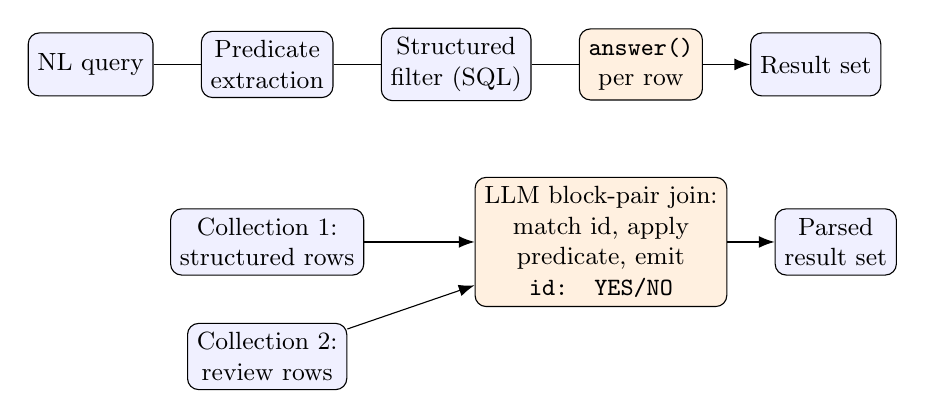
\begin{tikzpicture}[
  node distance=6mm and 6mm,
  box/.style={draw, rounded corners, align=center, minimum height=8mm, font=\small, fill=blue!6},
  llmbox/.style={draw, rounded corners, align=center, minimum height=8mm, font=\small, fill=orange!12},
  arr/.style={-{Latex[length=2mm]}}
]
\node[box] (q) {NL query};
\node[box, right=of q] (parse) {Predicate\\extraction};
\node[box, right=of parse] (sql) {Structured\\filter (SQL)};
\node[llmbox, right=of sql] (udf) {\texttt{answer()}\\per row};
\node[box, right=of udf] (out) {Result set};
\draw[arr] (q)--(parse)--(sql)--(udf)--(out);

\node[box, below=14mm of parse] (r1) {Collection 1:\\structured rows};
\node[box, below=6mm of r1] (r2) {Collection 2:\\review rows};
\node[llmbox, right=14mm of r1] (join) {LLM block-pair join:\\match id, apply\\predicate, emit\\\texttt{id: YES/NO}};
\node[box, right=of join] (out2) {Parsed\\result set};
\draw[arr] (r1) -- (join);
\draw[arr] (r2) -- (join);
\draw[arr] (join) -- (out2);
\end{tikzpicture}
}
\caption{Top: SUQL baseline (row-wise \texttt{answer()} after pushdown). Bottom: Trummer baseline -- no pushdown; the LLM joins a block of each collection and applies the predicate in one call.}
\label{fig:baselines}
\end{figure*}

\subsection{SUQL baseline: predicate pushdown}
Structured predicates are compiled to a \texttt{WHERE} clause and executed once against an in-memory SQLite instance. For every surviving row, one \texttt{answer(review, question)} call is issued to the LLM (Listing~\ref{lst:suql-prompt}), which returns \texttt{YES}/\texttt{NO}. Cost is $O(|R_\sigma|)$ calls, where $R_\sigma$ is the structurally filtered relation; quality is close to the ceiling because every row is judged individually, in full context, with an explicitly recall-first evidence-retrieval framing.

\begin{lstlisting}[style=prompt, caption={\texttt{answer()} system prompt, verbatim from the implementation (SUQL baseline).}, label={lst:suql-prompt}]
You are a recall-first semantic filter for movie reviews.
Decide whether the review provides evidence that the movie
satisfies the question. Answer YES for direct wording, a
synonym/paraphrase, a described example, or a reasonable
implication; count explicit mentions even when negated,
qualified, or critical (evidence retrieval, not sentiment
scoring). Answer NO when support is absent, generic, or
based only on genre/topic. Return exactly YES or NO.
\end{lstlisting}

\subsection{Trummer baseline: adaptive two-collection block join}
\label{sec:trummer-baseline}
Unlike the SUQL baseline, the Trummer baseline applies \emph{no} structural pushdown: the structured relation and the review relation are kept as two separate collections, partitioned independently into blocks, and the LLM is asked to join one block of each and apply the semantic predicate in a single call (Listing~\ref{lst:trummer-prompt}), returning one \texttt{movie\_id: YES/NO} decision per line. Block sizes are chosen by an adaptive tuning routine that also checks response coverage and re-partitions when a block's decisions are incomplete. Because the whole $100$-row candidate pool (not just the $40$ rows that satisfy $\sigma_S$) must be covered by block pairs, call counts scale with pool size and vary substantially with how often coverage checks trigger a retry ($30$--$268$ calls across our ten questions). Two systematic error sources follow directly from this design: (a) a block pair's response may echo a \texttt{movie\_id} that does not exactly match any input row (join/parsing drift), and (b) the model may decide only part of a block before drifting, undercounting true positives -- the dominant driver of the baseline's low recall.

\begin{lstlisting}[style=prompt, caption={Block-join prompt, verbatim from \texttt{operators.py} (Trummer baseline).}, label={lst:trummer-prompt}]
Find every movie in Collection 1 that has a review in
Collection 2 satisfying this predicate: {predicate}
Act as a recall-first semantic filter, while requiring
review-specific evidence. [...evidence-retrieval rules,
identical in spirit to Listing 1...]
A review belongs to a movie only when tconst is exactly
equal to movie_id. Return one decision per line as:
movie_id: YES or movie_id: NO.
Collection 1: {block_1_rows}
Collection 2: {block_2_rows}
Decisions:
\end{lstlisting}

\section{Cascaded Architectures (V1)}
\label{sec:cascade}

Both V1 variants add the same structural idea --- a \emph{two-level cascade} --- in front of the semantic operator of their respective baseline.

\begin{figure}[t]
\centering
\resizebox{\columnwidth}{!}{%
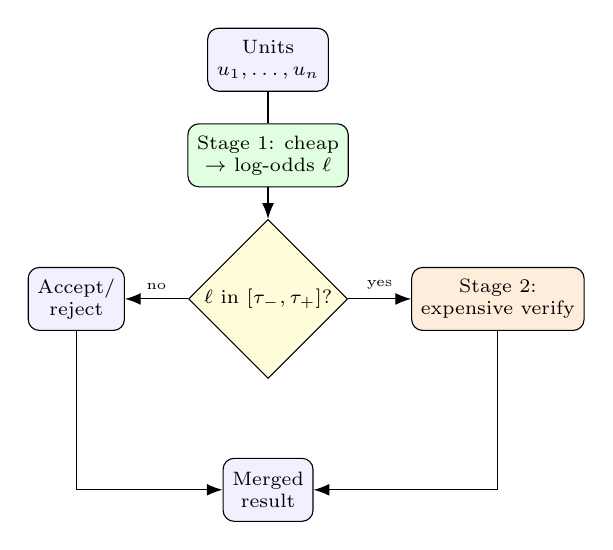
\begin{tikzpicture}[
  node distance=4mm and 4mm,
  box/.style={draw, rounded corners, align=center, minimum height=8mm, font=\scriptsize, fill=blue!6},
  cheap/.style={draw, rounded corners, align=center, minimum height=8mm, font=\scriptsize, fill=green!12},
  exp/.style={draw, rounded corners, align=center, minimum height=8mm, font=\scriptsize, fill=orange!14},
  dec/.style={draw, diamond, align=center, font=\scriptsize, fill=yellow!15, inner sep=1pt},
  arr/.style={-{Latex[length=2mm]}}
]
\node[box] (in) {Units\\$u_1,\dots,u_n$};
\node[cheap, below=of in] (cheap) {Stage 1: cheap\\$\to$ log-odds $\ell$};
\node[dec, below=of cheap] (dec) {$\ell$ in $[\tau_-,\tau_+]$?};
\node[exp, right=8mm of dec] (exp) {Stage 2:\\expensive verify};
\node[box, left=8mm of dec] (accept) {Accept/\\reject};
\node[box, below=10mm of dec] (out) {Merged\\result};
\draw[arr] (in)--(cheap)--(dec);
\draw[arr] (dec) -- node[above,font=\tiny]{yes} (exp);
\draw[arr] (dec) -- node[above,font=\tiny]{no} (accept);
\draw[arr] (exp) |- (out);
\draw[arr] (accept) |- (out);
\end{tikzpicture}
}
\caption{Two-level cascade shared by SUQL~V1 ($B{=}1$) and Trummer~V1 ($B{=}8$, batched).}
\label{fig:cascade}
\end{figure}

\subsection{SUQL~V1: cascaded predicate pushdown}
After structural pushdown, a cheap stage scores every surviving row with a single-token, logprob-based probe (\texttt{max\_tokens=1}; the log-odds is the difference of the model's own log-probabilities for the \texttt{1}/\texttt{0} completion tokens, not a self-reported number). Rows with $|\ell_i|$ outside the calibrated band are resolved without any further LLM call; only rows inside the band are escalated to a full \texttt{answer()} call. This is strictly a \emph{subset} of the row-wise baseline's LLM calls ($B{=}1$, one cheap call per row), so SUQL~V1 can only use fewer or equal \emph{expensive} calls than the baseline; wall-clock time can still grow substantially, because (\S\ref{sec:asymptotic-dominance}) the cheap stage's own per-row latency here exceeds the expensive stage's per-call latency -- a single-token completion still pays the full prompt-prefill cost of a review-length input.

\subsection{Trummer~V1: cascaded, structured, batched join}
\label{sec:trummer-v1}
Trummer~V1 (i) adds an explicit structured filter \emph{before} any LLM call -- the one variant in the Trummer family that gets SUQL-style pushdown; (ii) batches candidates ($B{=}8$ rows/call) and asks for a direct three-way \texttt{YES}/\texttt{NO}/\texttt{UNCERTAIN} label per row rather than a continuous score; (iii) re-verifies \texttt{UNCERTAIN} (or low-confidence) rows in a batched expensive pass. Its threshold is learned by a point-estimate agreement search rather than SUQL~V1's Beta-posterior bound (\S\ref{sec:beta-posterior}) -- unifying the two is future work. This is why Trummer~V1 is faster \emph{and} more accurate than its baseline at once: structural pushdown shrinks the pool before any call runs, batching amortizes prompt overhead across $8$ rows per call, and the verification pass repairs the join baseline's characteristic recall loss.

\begin{algorithm}[t]
\caption{Two-level cascaded semantic filter}
\label{alg:cascade}
\begin{algorithmic}[1]
\Require rows $R_\sigma$, predicate $P$, cheap scorer $f_1$, expensive operator $f_2$, calibration set $C$, target quality $Q^\ast$
\State $(\tau_-, \tau_+) \gets \textsc{CalibrateBand}(f_1, C, Q^\ast)$ \Comment{\S\ref{sec:cascade-math}}
\State $\mathit{Accept}, \mathit{Escalate} \gets \emptyset,\emptyset$
\For{$r \in R_\sigma$}
  \State $\ell \gets \operatorname{logit}(f_1(r, P))$
  \If{$\ell \ge \tau_+$} \State $\mathit{Accept} \gets \mathit{Accept} \cup \{r\}$
  \ElsIf{$\ell > \tau_-$} \State $\mathit{Escalate} \gets \mathit{Escalate} \cup \{r\}$
  \EndIf
\EndFor
\For{$r \in \mathit{Escalate}$} \Comment{Only ambiguous rows reach the LLM}
  \If{$f_2(r, P) = \textsc{Yes}$} \State $\mathit{Accept} \gets \mathit{Accept} \cup \{r\}$ \EndIf
\EndFor
\State \Return $\mathit{Accept}$
\end{algorithmic}
\end{algorithm}

\section{Calibrating the Cascade}
\label{sec:cascade-math}

\subsection{Log-odds scoring and the ambiguity band}
The cheap stage returns a probability $p_i \in (0,1)$; we work in log-odds space, $\ell_i = \log \frac{p_i}{1-p_i}$, additive under independent evidence combination and symmetric around the decision point $\ell_i=0$. We choose the band from a held-out calibration set $C$ ($|C|{=}20$ in our implementation) rather than a hand-picked $\epsilon$.

\subsection{Beta-posterior credible bounds}
\label{sec:beta-posterior}
Fix $\tau$, let $A_\tau = \{r \in C: \ell(r)\ge\tau\}$, and let $\mathit{TP}(\tau),\mathit{FN}(\tau)$ be its true/false positive/negative counts against ground truth. Under a Binomial model with a uniform Beta$(1,1)$ prior, the posterior recall is $r\mid \mathit{TP},\mathit{FN} \sim \mathrm{Beta}(1{+}\mathit{TP}(\tau), 1{+}\mathit{FN}(\tau))$. For confidence level $\alpha$, the lower credible bound is
\[
  \widehat{r}_{\alpha}(\tau) = \texttt{betaincinv}\bigl(1{+}\mathit{TP}(\tau),\, 1{+}\mathit{FN}(\tau),\, 1-\alpha\bigr),
\]
the $(1{-}\alpha)$-quantile, \emph{not} the $\alpha$-quantile -- an off-by-quantile error we caught only via a unit test against a synthetic confusion matrix with a known closed-form bound, since the implementation's \texttt{alpha} denotes the confidence level itself. The precision bound is symmetric, using $\mathrm{Beta}(1{+}\mathit{TP}(\tau),1{+}\mathit{FP}(\tau))$. The band is $\tau_+=\min\{\tau:\widehat p_\alpha(\tau)\ge Q^\ast\}$, $\tau_-=\max\{\tau:\widehat r_\alpha(\tau)\ge Q^\ast\}$.

\subsection{Operator ordering}
For $k$ independent selection operators with per-call cost $c_i$ and selectivity $s_i$ evaluated in short-circuit order, expected cost is minimized by ascending $c_i/(1-s_i)$ -- cheap, likely-to-reject operators first~\cite{eleet}. This justifies placing the (free) structural filter before the batched cheap pass, and that before the batched expensive verification, in Trummer~V1's pipeline.

\section{Theoretical Cost Analysis}
\label{sec:asymptotic-dominance}

We now prove precisely when calibrated cascading is guaranteed to cost less than an all-expensive baseline over the same $n$-row candidate pool, and instantiate the result with our measured system constants.

\textbf{Setup.} Let rows be i.i.d.\ draws given the structured predicate. Vanilla costs $c_e$ calls / $\tau_e$ seconds per row. The cascade costs $c_c/B$ calls and $\tau_c/B$ seconds per row (batching factor $B$), escalates each row independently with calibrated probability $\pi$, and pays a one-time calibration cost $K_{\mathrm{calls}}, K_{\mathrm{time}}$. With $S_n\sim\mathrm{Binomial}(n,\pi)$ escalations,
\[
  \mathrm{Calls}_{\mathrm{casc}}(n) = K_{\mathrm{calls}} + n\tfrac{c_c}{B} + S_n c_e,
\]
\[
  \mathrm{Time}_{\mathrm{casc}}(n) = K_{\mathrm{time}} + n\tfrac{\tau_c}{B} + S_n \tau_e.
\]

\begin{proposition}[Finite crossover]
\label{prop:crossover}
Let $\Delta_{\mathrm{calls}} = (1-\pi)c_e - c_c/B$. If $\Delta_{\mathrm{calls}}>0$, then $\mathbb E[\mathrm{Calls}_{\mathrm{casc}}(n)] < n c_e \iff n > n^\ast_{\mathrm{calls}} := K_{\mathrm{calls}}/\Delta_{\mathrm{calls}}$, and the gap grows unboundedly in $n$. If $\Delta_{\mathrm{calls}}\le 0$, no finite $n$ helps: the cascade is asymptotically worse. The symmetric statement holds for time with $\Delta_{\mathrm{time}}=(1-\pi)\tau_e-\tau_c/B$.
\end{proposition}
\begin{proof}
By linearity, $\mathbb E[\mathrm{Calls}_{\mathrm{casc}}(n)]=K_{\mathrm{calls}}+n(c_c/B+\pi c_e)$; $K_{\mathrm{calls}}+n(c_c/B+\pi c_e) < nc_e \iff n\Delta_{\mathrm{calls}} > K_{\mathrm{calls}}$.
\end{proof}

\begin{proposition}[Exponentially vanishing failure probability]
\label{prop:hoeffding}
For $n>n^\ast_{\mathrm{calls}}$, let $t_n=(n\Delta_{\mathrm{calls}}-K_{\mathrm{calls}})/c_e>0$. Then
$\Pr[\mathrm{Calls}_{\mathrm{casc}}(n)\ge nc_e] \le \exp(-2t_n^2/n)$, which is $O(e^{-cn})$ for a constant $c=2\Delta_{\mathrm{calls}}^2/c_e^2$.
\end{proposition}
\begin{proof}
The event equals $\{S_n \ge n\pi+t_n\}$; $S_n$ is a sum of $n$ i.i.d.\ bounded variables with mean $n\pi$, so Hoeffding's inequality gives the bound; $t_n$ is linear in $n$, so the exponent is $\Theta(n)$.
\end{proof}

Together, Propositions~\ref{prop:crossover}--\ref{prop:hoeffding} give the precise sense in which ``enough rows'' make cascading win: a finite, computable crossover in expectation, and an exponentially shrinking failure probability for any single realized run beyond it.

\begin{table}[t]
\centering\scriptsize
\begin{tabular}{lrr}
\toprule
Quantity & SUQL~V1 & Trummer~V1 \\
\midrule
Batching factor $B$ & $1$ & $8$ \\
Escalation rate $\pi$ & $0.751$ & $0.125$ \\
Cheap cost/row $\tau_c/B$ (s) & $20.86$ & $0.527$ \\
Expensive cost/call $\tau_e$ (s) & $2.97$ & $2.80$ \\
$K_{\mathrm{calls}}$ (calibration) & $20$ & $1$ \\
$\Delta_{\mathrm{calls}}=(1-\pi)-1/B$ & $-0.751$ & $+0.750$ \\
$\Delta_{\mathrm{time}}$ (s) & $-20.12$ & $+1.919$ \\
$n^\ast_{\mathrm{calls}}$ & none & $\approx 1.3$ \\
\bottomrule
\end{tabular}
\caption{Measured constants (\S\ref{sec:eval}) in Prop.~\ref{prop:crossover}, using a ``lean vanilla'' reference ($c_e{=}1$ call/row) to isolate the cascade mechanism from baseline-specific overhead (e.g.\ SUQL baseline's \texttt{summary()} calls).}
\label{tab:theory-constants}
\end{table}

Table~\ref{tab:theory-constants} shows both margins are \emph{negative} for SUQL~V1: with no batching ($B{=}1$) and a $75\%$ escalation rate, its cheap stage cannot beat a lean, single-call-per-row vanilla on calls, and its measured per-row latency ($20.86$s) already exceeds the expensive stage's own per-call latency ($2.97$s), so no finite pool size rescues it on time -- exactly matching the observed $8\times$ wall-time regression (\S\ref{sec:results}). Trummer~V1's margins are comfortably positive: batching ($B{=}8$) drives its effective per-row cheap cost to $0.527$s, an order of magnitude below the expensive per-call cost, and its low escalation rate ($12.5\%$) plus a tiny, already-batched calibration cost give a call-count crossover of $n^\ast\approx 1.3$ rows -- the cascade is predicted to win almost immediately, matching what we observe even at the modest $n{=}40$ used here. \textbf{Batching the cheap stage is therefore not an implementation detail: it determines whether the margin condition can hold at all}, and is accordingly the most consequential remaining change for SUQL~V1 (\S\ref{sec:future}).

\section{Experimental Setup}
\label{sec:eval}
\textbf{Dataset.} Ten held-out, genre-diverse questions (\texttt{10q} suite), each with its own controlled, auditable $100$-movie pool drawn from a $\sim$25{,}000-row canonical IMDb corpus: $12$ true positives, $28$ structured-semantic negatives, $30$ semantic-only distractors, $30$ double negatives; $40$ rows satisfy the structured predicate in every question.
\textbf{Models.} Ollama-served open-weight models (cheap: Gemma~4 \texttt{e2b}; expensive: Gemma~4 \texttt{26b}) behind a LiteLLM abstraction layer.
\textbf{Repetitions.} Each of the four methods is run $10\times$ per question; we report means over all $10{\times}10$ runs (\texttt{aggregate.csv}) and per-question means (\texttt{comparison.csv}).
\textbf{Metrics.} Precision, recall, F1 against an annotation-derived gold set; wall-clock time; LLM calls (with cheap/expensive split for cascades).

\section{Results}
\label{sec:results}

\begin{table}[t]
\caption{Cost per question, averaged over 10 questions $\times$ 10 reps.}
\label{tab:cost}
\centering\footnotesize
\resizebox{\linewidth}{!}{%
\begin{tabular}{lrrrr}
\toprule
Metric & SUQL base. & SUQL V1 & Trummer base. & \textbf{Trummer V1} \\
\midrule
Wall time (s) & 115.57 & 923.60 & 71.28 & \textbf{35.05} \\
LLM calls     & 117.08 & 70.05 & 96.87 & \textbf{10.00} \\
\bottomrule
\end{tabular}}
\end{table}

\begin{table}[t]
\caption{Quality per question (best variant per row in bold).}
\label{tab:quality}
\centering\footnotesize
\resizebox{\linewidth}{!}{%
\begin{tabular}{lrrrr}
\toprule
Metric & SUQL base. & SUQL V1 & Trummer base. & \textbf{Trummer V1} \\
\midrule
Precision & 0.683 & 0.709 & 0.655 & \textbf{0.810} \\
Recall    & 0.758 & \textbf{0.808} & 0.408 & 0.750 \\
F1        & 0.678 & 0.696 & 0.444 & \textbf{0.757} \\
\bottomrule
\end{tabular}}
\end{table}

Cascading the row-wise strategy (SUQL~V1) trades time for a modest quality gain: $7.99\times$ slower wall time (ambiguous rows now pay for both stages, and Table~\ref{tab:theory-constants} shows why this is structural, not incidental) for $+2.7\%$ F1 and $+6.6\%$ recall. The join baseline is far cheaper than both SUQL variants but at a real quality cost (F1 $0.444$, worst of the four, driven by recall $0.408$). Cascading the join strategy (Trummer~V1) improves \emph{both} axes over its own baseline ($2.03\times$ faster, $10\times$ fewer calls, $+70\%$ F1) and, relative to SUQL~V1, is $26.3\times$ faster and uses $1/7$ the calls while still gaining $+8.8\%$ F1 and $+14.2\%$ precision, at a $\approx 7\%$ relative recall cost.

\textbf{Robustness across questions.} Per-question F1 ranges from $0.267$--$0.917$ (SUQL baseline), $0.286$--$0.957$ (SUQL~V1), $0.154$--$0.667$ (Trummer baseline), and $0.500$--$0.917$ (Trummer~V1). Trummer~V1's \emph{floor} is the highest of the four -- it is the only method that does not collapse on the hardest question in the suite (romance-chemistry, Q3: SUQL baseline $0.267$, Trummer baseline $0.154$, SUQL~V1 $0.286$, Trummer~V1 $0.917$), consistent with the batched escalation step repairing exactly the paraphrase-heavy, vocabulary-mismatched cases both baselines struggle with.

\clearpage
\begin{figure}[tb]
\centering

\includegraphics[width=\columnwidth]{figs/imdb10q/01_quality.png}
\caption{IMDb \texttt{10q}: precision, recall, F1 by method.}
\label{fig:imdb-quality}
\end{figure}

Figure~\ref{fig:imdb-quality}: SUQL~V1 has the tallest recall bar ($0.808$); Trummer baseline is weakest throughout, recall collapsing to $0.408$ against comparable precision ($0.655$) -- the incomplete-coverage failure mode of \S\ref{sec:trummer-baseline}. Trummer~V1's F1 (purple) is tallest of the four.

\begin{figure}[tb]
\centering

\includegraphics[width=\columnwidth]{figs/imdb10q/02_time.png}
\caption{IMDb \texttt{10q}: mean wall time, cheap vs.\ expensive stage.}
\label{fig:imdb-time}
\end{figure}

Figure~\ref{fig:imdb-time} is the clearest single visual of Table~\ref{tab:theory-constants}'s mechanism: SUQL~V1's bar is tallest ($923.6$s) and \emph{dominated by its own cheap stage} (green, $77\%$) -- the cheap probe is not actually cheap in wall time. Trummer~V1's bar is shortest ($35.1$s).

\begin{figure}[tb]
\centering

\includegraphics[width=\columnwidth]{figs/imdb10q/03_calls.png}
\caption{IMDb \texttt{10q}: mean LLM calls, cheap vs.\ expensive stage.}
\label{fig:imdb-calls}
\end{figure}

Figure~\ref{fig:imdb-calls}: SUQL~V1's calls ($70.0$) are \emph{lower} than baseline's ($117.1$), unlike the time comparison above -- SUQL~V1 trades calls for time, not both. Trummer~V1 needs only $10.0$ calls, split evenly cheap/expensive.

\begin{figure*}[t]
\centering

\includegraphics[width=0.55\textwidth]{figs/imdb10q/04_best_solution.png}
\caption{IMDb \texttt{10q}: recall vs.\ wall time; harness best-solution annotation is Trummer~V1.}
\label{fig:imdb-best}
\end{figure*}

Figure~\ref{fig:imdb-best} plots recall against time for all four methods at once: Trummer~V1 (outlined) sits bottom-left (low time, competitive recall), while SUQL~V1 sits far right ($923.6$s) at similar recall to SUQL baseline -- isolating SUQL~V1's time regression from its recall profile.

\begin{figure}[tb]
\centering

\includegraphics[width=\columnwidth]{figs/imdb10q/05_cost_by_approach.png}
\caption{IMDb \texttt{10q}: estimated \$-cost per question.}
\label{fig:imdb-cost}
\end{figure}

Figure~\ref{fig:imdb-cost}: at \$3/accelerator-hour, SUQL~V1 costs \$0.770/question -- $26\times$ Trummer~V1's \$0.029. Per-call figures show the cheap stage costing \emph{more} per call than expensive for both cascades ($7.0\times$ SUQL~V1, $1.5\times$ Trummer~V1) -- exactly the time ratios of Table~\ref{tab:theory-constants}, since \$-cost here is simply time $\times$ a flat rate.

\begin{figure}[tb]
\centering

\includegraphics[width=\columnwidth]{figs/imdb10q/06_cost_vs_f1.png}
\caption{IMDb \texttt{10q}: cost--F1 Pareto frontier.}
\label{fig:imdb-pareto}
\end{figure}

Figure~\ref{fig:imdb-pareto} shows \textbf{Trummer~V1 as the unique non-dominated point}: lowest cost \emph{and} highest F1 simultaneously, so it alone strictly dominates all three other methods (unlike the Amazon results below, where two points share the frontier) -- and resolves, rather than merely flags, the cross-model \$-cost puzzle noted below.

\section{Discussion}
\label{sec:discussion}

\textbf{Selectivity still dominates.} Every question in this suite fixes structural selectivity at $40\%$ ($40$ of $100$ rows); the ranking we report is most informative at that selectivity and should be re-measured across a selectivity sweep before being treated as universal.

\textbf{The \texttt{answer()} yield rate as a diagnostic.} The fraction of structurally-filtered rows accepted by the semantic operator remains a label-free predicate-quality signal: very high yield indicates an under-specified predicate; very low yield suggests over-constraint or vocabulary mismatch.

\textbf{\texttt{LIMIT} without early termination.} None of the four implementations currently stop evaluating early once a \texttt{LIMIT k} target is met, despite Algorithm~\ref{alg:cascade} supporting it in principle.

\textbf{Threats to validity.} All ten questions share the same $100/40/12$ structural shape by design; this isolates semantic-task difficulty as the varying factor but leaves a selectivity sweep (the repository's \texttt{1q}/\texttt{3q}/\texttt{5q} suites, and a still-larger suite) as the natural next step.

\section{Cross-Domain Validation: Amazon Data}
\label{sec:amazon}

Three Amazon experiments test whether findings above are IMDb-specific: (1) a wide pool-size sweep ($n{=}100$--$300$, Gemma, one question) stress-testing Proposition~\ref{prop:crossover} directly; (2) a full ten-question \emph{Amazon Fashion} suite, same Gemma pair, same \texttt{10q} format as IMDb; (3) a five-question Amazon suite under Qwen.

\textbf{IMDb vs.\ Amazon Fashion (matched suite, same model).} Table~\ref{tab:imdb-vs-amazon} compares the two \texttt{10q} suites directly -- a materially better comparison than a single pool-size point used in an earlier revision of this paper, which it corrects: with the full ten-question average, \textbf{Trummer~V1's F1 gain over SUQL baseline does not replicate on Amazon Fashion} (a small $-4.3\%$, not a gain). SUQL baseline itself is far cheaper on Amazon Fashion ($49.2$ vs.\ $117.1$ calls), leaving less headroom for the cascade; more importantly, \textbf{SUQL~V1 is strictly dominated by its own baseline here} -- worse on calls ($+59\%$), time ($+148\%$), \emph{and} F1 ($-7.1\%$) at once, unlike IMDb where it at least traded time for quality.

\begin{table}[t]
\centering\footnotesize
\begin{tabular}{lrr}
\toprule
 & IMDb \texttt{10q} & Amazon Fashion \texttt{10q} \\
\midrule
\multicolumn{3}{l}{\emph{Trummer~V1 vs.\ SUQL baseline}} \\
$\Delta$F1    & $+11.7\%$ & $-4.3\%$ \\
$\Delta$calls & $-91.5\%$ & $-73.6\%$ \\
$\Delta$time  & $-69.7\%$ & $-39.8\%$ \\
\midrule
\multicolumn{3}{l}{\emph{SUQL~V1 vs.\ SUQL baseline}} \\
$\Delta$F1    & $+2.7\%$  & $-7.1\%$ \\
$\Delta$calls & $-40.2\%$ & $+59.1\%$ \\
$\Delta$time  & $+699\%$  & $+148\%$ \\
\bottomrule
\end{tabular}
\caption{Same model, same suite design, different domain.}
\label{tab:imdb-vs-amazon}
\end{table}

\clearpage
\begin{figure}[tb]
\centering

\includegraphics[width=\columnwidth]{figs/amazon_fashion_gemma/01_quality.png}
\caption{Amazon Fashion \texttt{10q}, Gemma: precision, recall, F1.}
\label{fig:amzf-quality}
\end{figure}

Figure~\ref{fig:amzf-quality}: three of four F1 bars sit in a much narrower band ($0.776$--$0.835$) than on IMDb. The exception is Trummer baseline, whose precision collapses to $0.330$ despite the \emph{highest} recall seen so far ($0.967$) -- the opposite imbalance from its IMDb profile.

\begin{figure}[tb]
\centering

\includegraphics[width=\columnwidth]{figs/amazon_fashion_gemma/02_time.png}
\caption{Amazon Fashion \texttt{10q}, Gemma: mean wall time, cheap vs.\ expensive stage.}
\label{fig:amzf-time}
\end{figure}

Figure~\ref{fig:amzf-time} repeats IMDb's pattern (Figure~\ref{fig:imdb-time}): SUQL~V1 tallest ($48.7$s, $77\%$ cheap-stage), Trummer~V1 shortest ($11.8$s). SUQL baseline itself is much cheaper here ($19.6$s vs.\ $115.6$s), so the \emph{relative} speedup is weaker.

\begin{figure}[tb]
\centering

\includegraphics[width=\columnwidth]{figs/amazon_fashion_gemma/03_calls.png}
\caption{Amazon Fashion \texttt{10q}, Gemma: mean LLM calls, cheap vs.\ expensive stage.}
\label{fig:amzf-calls}
\end{figure}

Figure~\ref{fig:amzf-calls}: SUQL~V1's bar ($78.3$ calls) is \emph{taller} than baseline's ($49.2$) -- the reverse of IMDb (Figure~\ref{fig:imdb-calls}), where SUQL~V1 used fewer calls. Trummer~V1 again needs the fewest ($13.0$).

\begin{figure*}[t]
\centering

\includegraphics[width=0.55\textwidth]{figs/amazon_fashion_gemma/04_best_solution.png}
\caption{Amazon Fashion \texttt{10q}, Gemma: recall vs.\ wall time; best-solution annotation is Trummer~V1.}
\label{fig:amzf-best}
\end{figure*}

Figure~\ref{fig:amzf-best}: SUQL~V1 sits far right on time while its recall bubble is no higher than baseline's or Trummer~V1's -- it buys no recall advantage for its much larger time cost here, unlike IMDb.

\begin{figure}[tb]
\centering

\includegraphics[width=\columnwidth]{figs/amazon_fashion_gemma/05_cost_by_approach.png}
\caption{Amazon Fashion \texttt{10q}, Gemma: estimated \$-cost per question.}
\label{fig:amzf-cost}
\end{figure}

Figure~\ref{fig:amzf-cost}: SUQL~V1 is the most expensive method (\$0.0406) despite Trummer baseline having no cheap stage at all (\$0.0306) -- SUQL~V1's extra calls and pricier cheap stage compound. Trummer~V1 remains cheapest (\$0.0098).

\begin{figure}[tb]
\centering

\includegraphics[width=\columnwidth]{figs/amazon_fashion_gemma/06_cost_vs_f1.png}
\caption{Amazon Fashion \texttt{10q}, Gemma: cost--F1 Pareto frontier.}
\label{fig:amzf-pareto}
\end{figure}

Figure~\ref{fig:amzf-pareto} shows \emph{two} non-dominated points -- Trummer~V1 and SUQL baseline -- rather than IMDb's single dominant point: SUQL baseline has slightly higher F1 ($0.835$ vs.\ $0.799$) at slightly higher cost ($\$0.0164$ vs.\ $\$0.0098$), so neither dominates the other.

\textbf{Scaling and reliability validation.} Computing $\Pr[\text{cascade cost}\ge\text{vanilla cost}]$ via full pairwise comparison across the $n{=}100$--$300$ sweep: on calls, the cascade lost \emph{zero} times at every $n$, in both the standard and adversarial ($K{\propto}n$) calibration regime. On time, one small ($0.66\%$) failure appears at $n{=}100$, vanishing by $n{=}125$ -- system-timing jitter, not the escalation-count randomness Proposition~\ref{prop:hoeffding} formalizes (\texttt{expensive\_calls} had zero within-$n$ variance here, so this confirms Prop.~\ref{prop:crossover}'s conclusion without exercising Prop.~\ref{prop:hoeffding}'s specific mechanism). Quality is less clean: Trummer~V1 loses F1 to vanilla at $2$--$4$ of $6$ pool sizes across the two regimes, tracking a \texttt{calibration\_agreement} that misses its $0.9$ target everywhere tested ($0.27$--$0.89$) -- reinforcing the case for porting SUQL~V1's Beta-posterior bound to Trummer~V1.

\clearpage
\begin{figure}[tb]
\centering
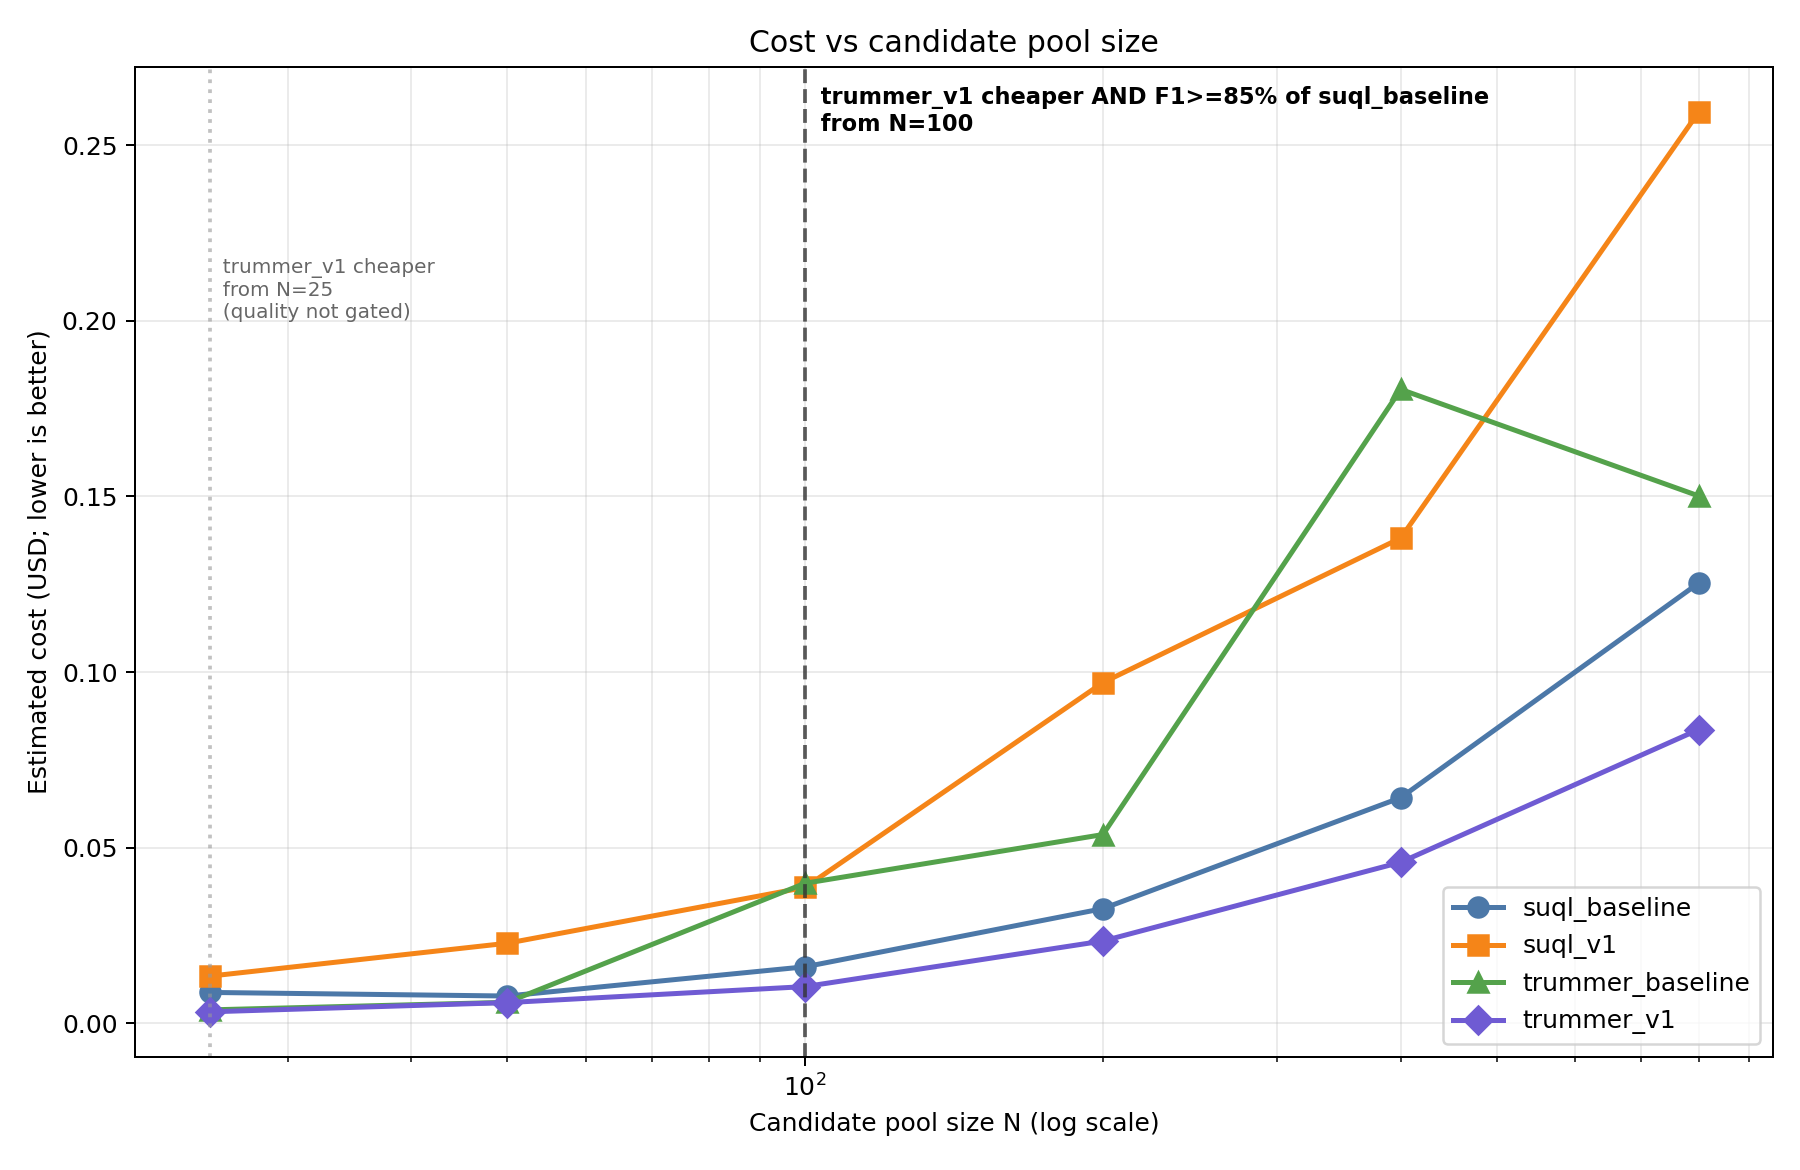
\includegraphics[width=\columnwidth]{figs/amazon/01_cost_vs_n.png}
\caption{\$-cost vs.\ pool size $n$ (log scale), all four methods.}
\label{fig:amzscale-cost}
\end{figure}

Figure~\ref{fig:amzscale-cost}: the near-flat-then-rising shape is the expected signature of a cost linear in $n$ viewed against $\log n$ (Prop.~\ref{prop:crossover}), not super-linear growth. Annotated thresholds mark where Trummer~V1 becomes cheaper ($n{=}25$) and cheaper \emph{and} within $85\%$ of baseline F1 ($n{=}100$).

\begin{figure}[tb]
\centering
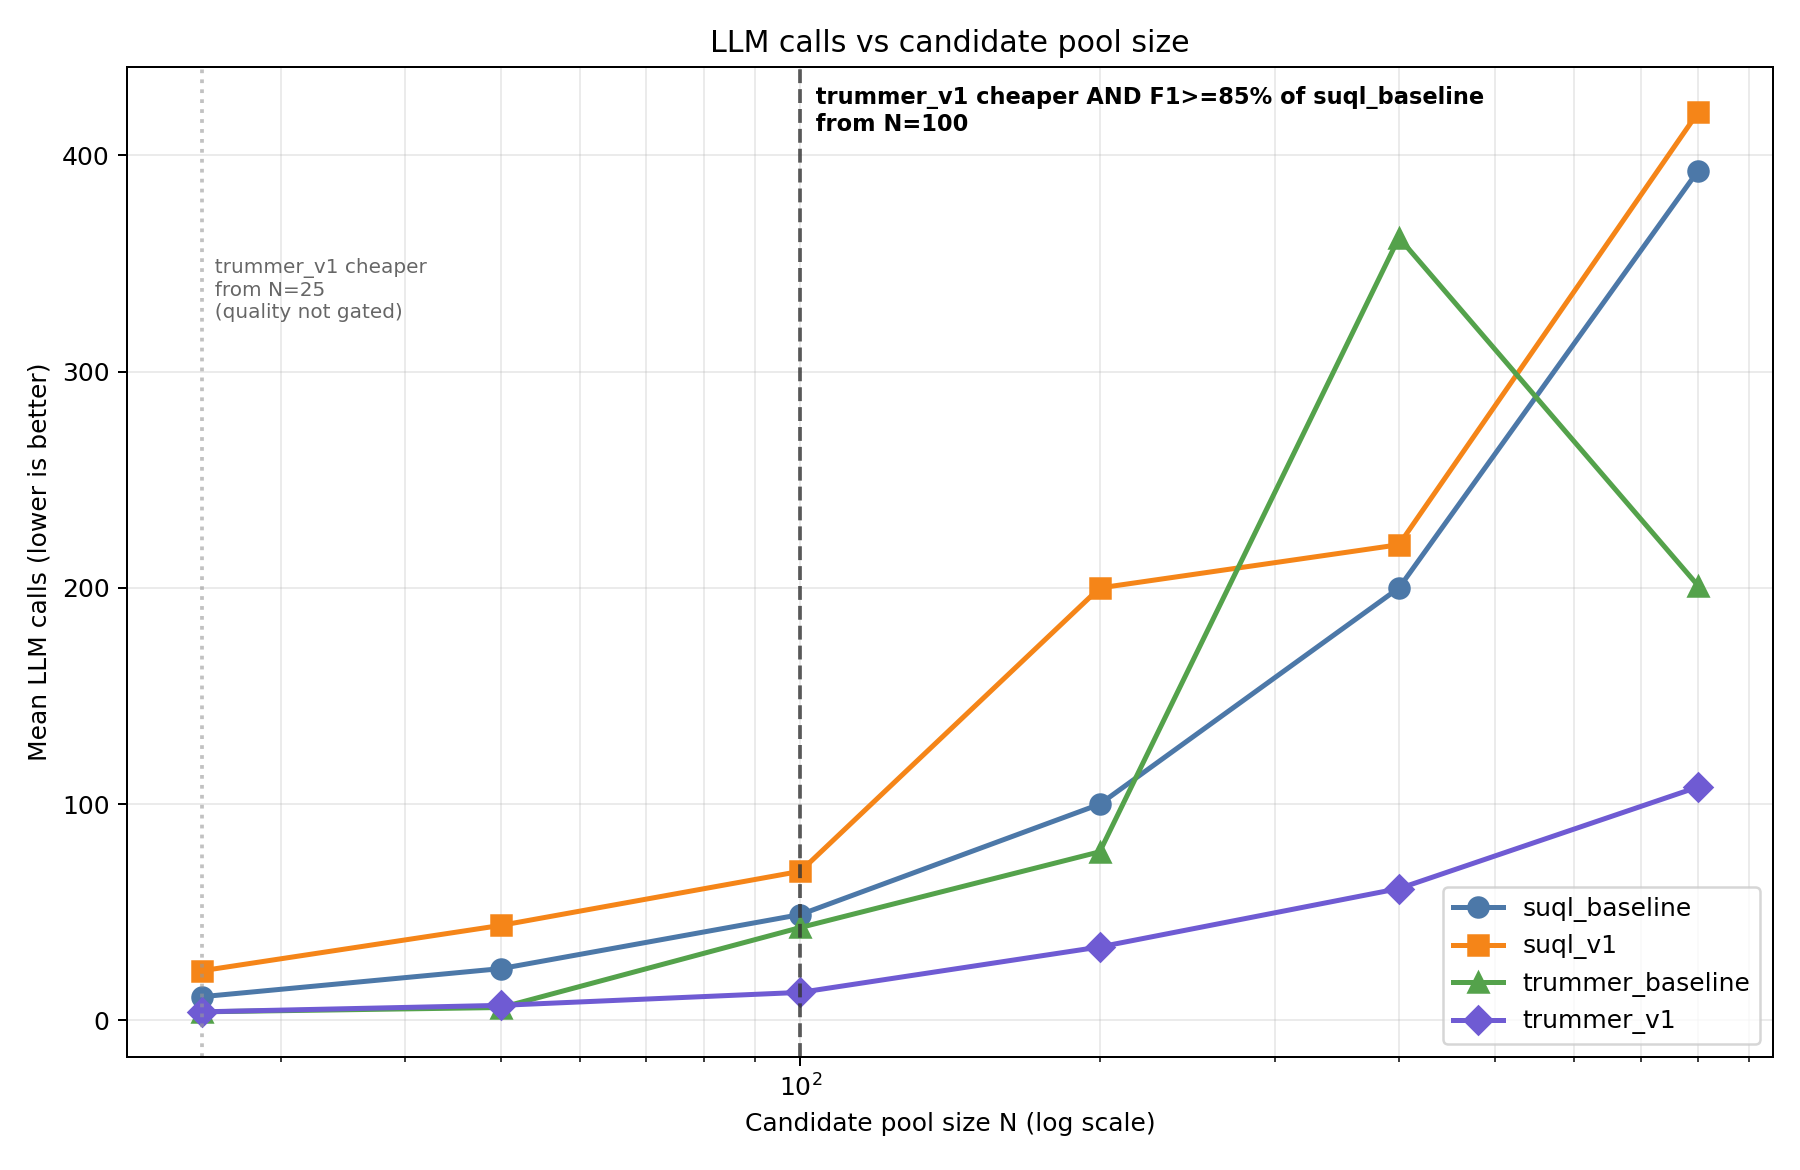
\includegraphics[width=\columnwidth]{figs/amazon/02_calls_vs_n.png}
\caption{Mean LLM calls vs.\ pool size $n$ (log scale).}
\label{fig:amzscale-calls}
\end{figure}

Figure~\ref{fig:amzscale-calls}: Trummer~V1 (purple) is lowest at every $n$; Trummer baseline (green) is visibly noisiest, consistent with its adaptive block-pairing retrying on parse failure (\S\ref{sec:trummer-baseline}).

\begin{figure}[tb]
\centering
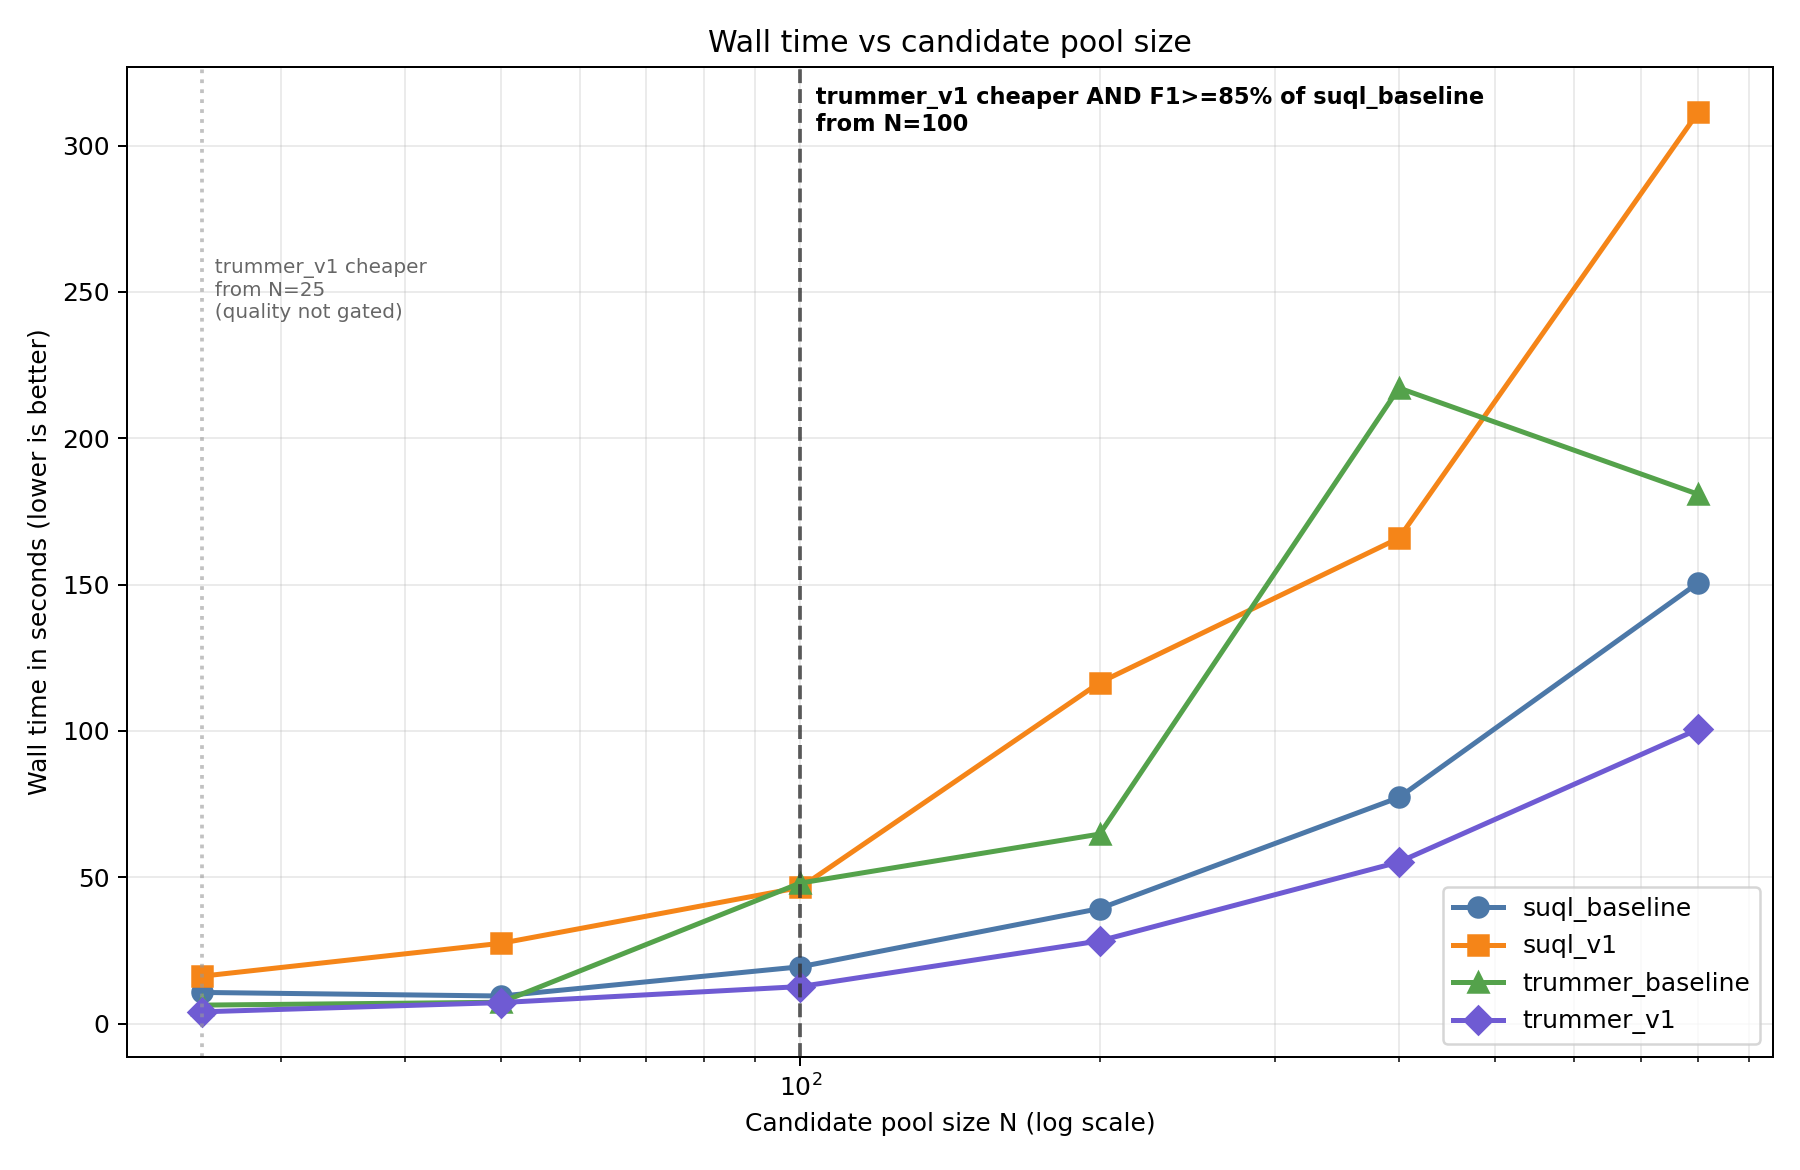
\includegraphics[width=\columnwidth]{figs/amazon/03_time_vs_n.png}
\caption{Mean wall time (s) vs.\ pool size $n$ (log scale).}
\label{fig:amzscale-time}
\end{figure}

Figure~\ref{fig:amzscale-time}: SUQL~V1 (orange) crosses above even noisy Trummer baseline by $n{\approx}150$ and finishes slowest at $n{=}300$ -- the same story as IMDb, now shown continuously across pool sizes.

\begin{figure}[tb]
\centering
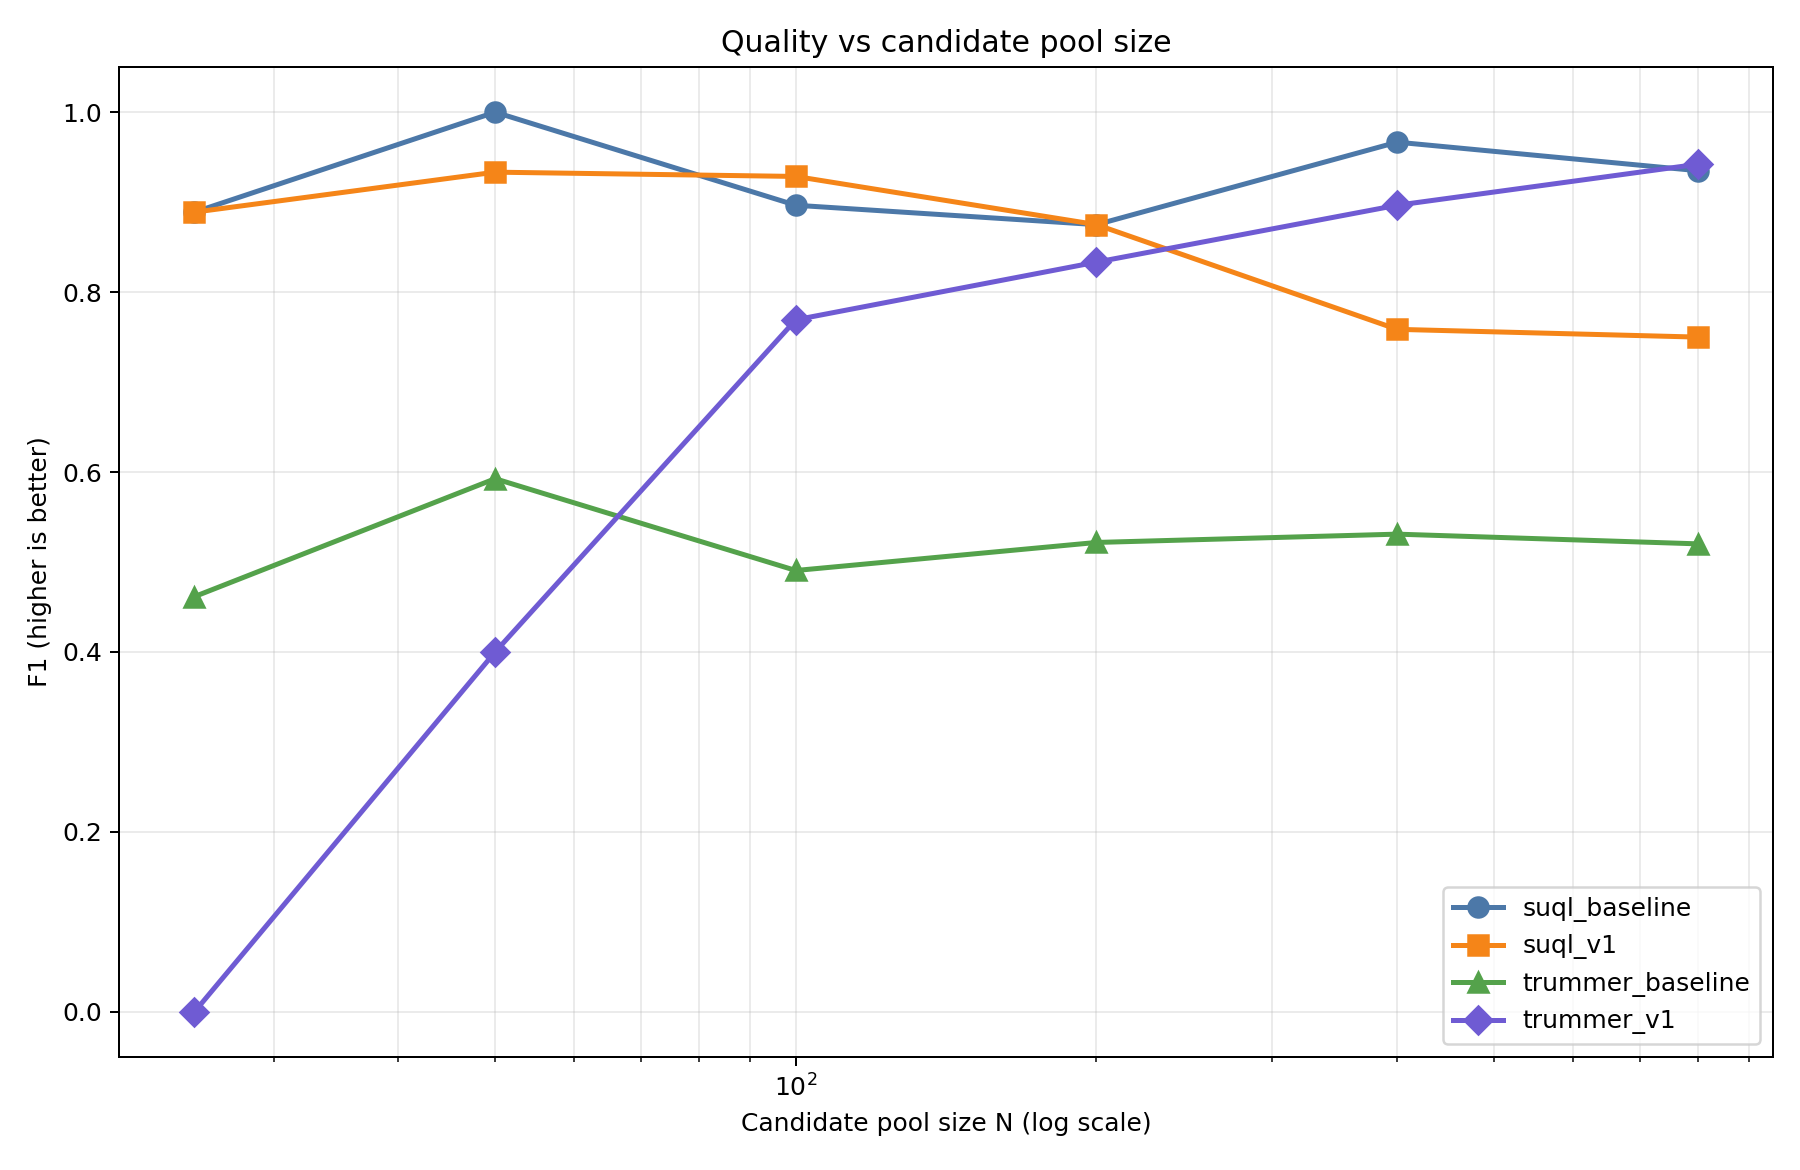
\includegraphics[width=\columnwidth]{figs/amazon/04_f1_vs_n.png}
\caption{F1 vs.\ pool size $n$ (log scale).}
\label{fig:amzscale-f1}
\end{figure}

Figure~\ref{fig:amzscale-f1} is the least monotonic: Trummer~V1 (purple) starts at F1${}=0$ at the smallest pool before climbing above every other method by $n{\gtrsim}150$ -- $\pi$ is not perfectly stable across differently-sized pools, and at the smallest $n$ the calibration set is too small relative to $n$ for the threshold search to produce a usable band.

\textbf{Qwen vs.\ Gemma.} A Qwen pair on the same Amazon workload (five-question suite) compares against the Amazon Fashion \texttt{10q} Gemma run above -- better-matched than the pool-size point used previously (which showed a small \emph{positive} Gemma F1 delta; the properly-averaged comparison shows a small \emph{negative} one, consistent with Qwen -- a correction, not silently revised). Both families agree in direction on every metric: Trummer~V1 trades a small, consistent F1 loss ($1.5$--$4.3\%$) for a large, consistent call reduction ($74$--$81\%$); SUQL~V1 is strictly dominated by its own baseline under \emph{both} models. This is the clearest cross-model evidence that the cost mechanism is architectural and portable, while SUQL~V1's unbatched design is the outlier. The earlier-noted near-identical SUQL~V1 \$-costs across the two runs (cheap $\$0.00062$ both; expensive $\$0.00036$ vs.\ $\$0.00033$) is now resolved rather than merely flagged: as confirmed above, \$-cost here is simply recorded time $\times$ a flat rate with no per-model pricing, so similar \$-costs reflect similar per-call \emph{latency}, not a shared underlying model.

\clearpage
\begin{figure}[tb]
\centering

\includegraphics[width=\columnwidth]{figs/qwen_amazon/01_quality.png}
\caption{Qwen, Amazon 5-question suite: precision, recall, F1 (error bars: std.\ dev.).}
\label{fig:qwen-quality}
\end{figure}

Figure~\ref{fig:qwen-quality}: Trummer baseline shows the same precision/recall imbalance under Qwen as under Gemma ($0.360$ precision, $0.907$ recall). The other three methods cluster tightly ($0.863$--$0.878$ F1) with overlapping error bars.

\begin{figure}[tb]
\centering

\includegraphics[width=\columnwidth]{figs/qwen_amazon/02_time.png}
\caption{Qwen, Amazon 5-question suite: mean wall time, cheap vs.\ expensive stage.}
\label{fig:qwen-time}
\end{figure}

Figure~\ref{fig:qwen-time}: SUQL~V1 tallest ($48.3$s, $77\%$ cheap-stage), Trummer~V1 shortest ($17.4$s) -- the same ranking as both Gemma runs, now under a different model family.

\begin{figure}[tb]
\centering

\includegraphics[width=\columnwidth]{figs/qwen_amazon/03_calls.png}
\caption{Qwen, Amazon 5-question suite: mean LLM calls, cheap vs.\ expensive stage.}
\label{fig:qwen-calls}
\end{figure}

Figure~\ref{fig:qwen-calls}: SUQL~V1 uses \emph{more} calls than baseline ($75.0$ vs.\ $48.6$), matching its Amazon-Fashion behavior under Gemma rather than its IMDb behavior.

\begin{figure*}[t]
\centering

\includegraphics[width=0.55\textwidth]{figs/qwen_amazon/04_best_solution.png}
\caption{Qwen, Amazon 5-question suite: recall vs.\ wall time; best-solution annotation is Trummer~V1.}
\label{fig:qwen-best}
\end{figure*}

Figure~\ref{fig:qwen-best}: SUQL baseline, Trummer baseline, and Trummer~V1 sit at broadly similar recall; SUQL~V1 alone is pulled far right on time -- the same isolated-outlier pattern as both Gemma figures.

\begin{figure}[tb]
\centering

\includegraphics[width=\columnwidth]{figs/qwen_amazon/05_cost_by_approach.png}
\caption{Qwen, Amazon 5-question suite: estimated \$-cost per question.}
\label{fig:qwen-cost}
\end{figure}

Figure~\ref{fig:qwen-cost}: SUQL~V1 is most expensive (\$0.0403), Trummer~V1 cheapest (\$0.0145). SUQL~V1's cheap-call cost here (\$0.00062) matches its Gemma/Amazon-Fashion counterpart to five significant figures -- the basis of the \$-cost puzzle resolved above.

\begin{figure}[tb]
\centering

\includegraphics[width=\columnwidth]{figs/qwen_amazon/06_cost_vs_f1.png}
\caption{Qwen, Amazon 5-question suite: cost--F1 Pareto frontier.}
\label{fig:qwen-pareto}
\end{figure}

Figure~\ref{fig:qwen-pareto} shows the same two-point frontier shape as Gemma/Amazon-Fashion: Trummer~V1 (\$0.0145, F1 $0.865$) and SUQL baseline (\$0.0175, F1 $0.878$) both non-dominated; SUQL~V1 and Trummer baseline each dominated on both axes.

\emph{Remaining scope}: neither run records model parameter counts, so $P_c/P_e$ cannot yet be stated for Qwen the way Table~\ref{tab:theory-constants} does for Gemma; both families now cover all four methods on Amazon data, closing the earlier coverage gap.

\section{Conclusion and Future Work}
\label{sec:future}
Across ten held-out, genre-diverse questions, a calibrated two-level cascade applied to a structurally-filtered, batched-join semantic operator (Trummer~V1) dominates both a row-wise pushdown baseline and its own uncascaded baseline on cost, F1, and worst-case robustness, at a small, quantified recall cost. We proved this dominance is not incidental: Proposition~\ref{prop:crossover} gives an exact margin condition on the cheap stage's batching factor and calibrated escalation rate, and Table~\ref{tab:theory-constants} shows the measured system satisfies it for Trummer~V1 and fails it for SUQL~V1 -- correctly predicting the $8\times$ wall-time regression the latter exhibits. \textbf{Batching SUQL~V1's currently row-wise cheap stage} is therefore the single most consequential remaining change, identified by theory rather than only by observation. Other near-term work: porting the Beta-posterior calibration bound to Trummer~V1 (currently a point-estimate agreement search); amortizing the one-time calibration cost across repeated invocations of the same predicate; and extending the benchmark across a selectivity sweep. Stretto's KV-cache-aware execution ladder (\emph{Expected Attention Press}) remains deferred pending a migration from Ollama to a backend exposing attention state directly (e.g.\ \texttt{vllm}).

\begin{thebibliography}{9}
\bibitem{suql} S.~Liu et al. SUQL: Conversational Search over Structured and Unstructured Data with Large Language Models. arXiv:2311.09818, 2023.
\bibitem{eleet} M.~Urban and C.~Binnig. ELEET: Efficient Learned Query Execution over Text and Tables. Proc.\ VLDB Endow., 2024.
\bibitem{stretto} G.~Sanmartino et al. Stretto: Bayesian Threshold Calibration and Cache-Aware Cascades for LLM Query Operators. arXiv:2602.04430v2, 2025.
\end{thebibliography}

\end{document}
